\documentclass{standalone}
\usepackage{tikz}
\begin{document}
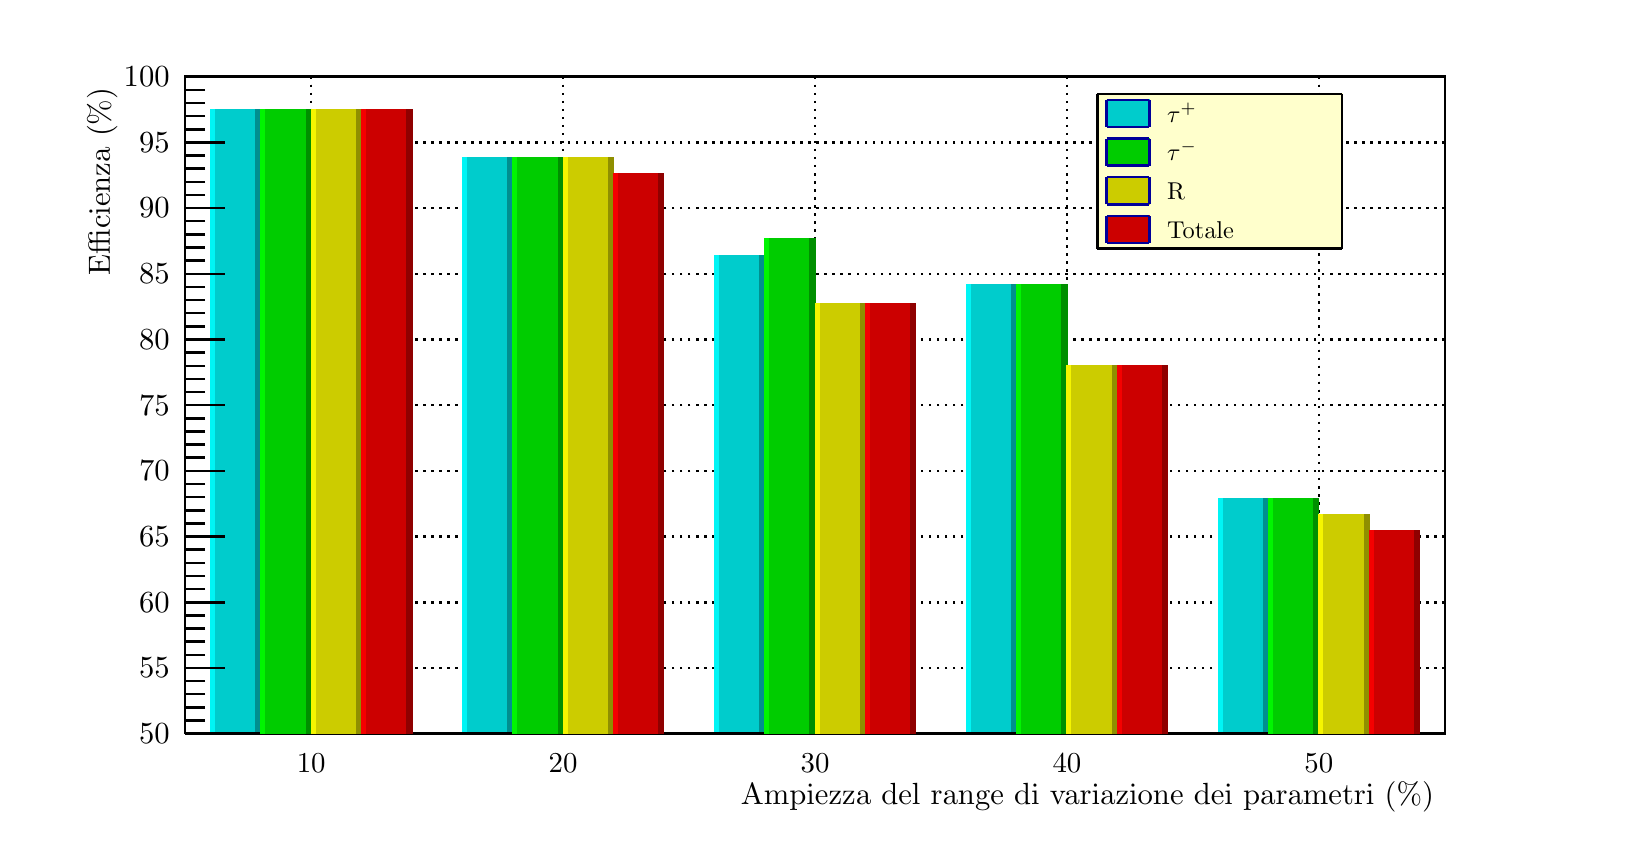
\begin{tikzpicture}
\pgfdeclareplotmark{cross} {
\pgfpathmoveto{\pgfpoint{-0.3\pgfplotmarksize}{\pgfplotmarksize}}
\pgfpathlineto{\pgfpoint{+0.3\pgfplotmarksize}{\pgfplotmarksize}}
\pgfpathlineto{\pgfpoint{+0.3\pgfplotmarksize}{0.3\pgfplotmarksize}}
\pgfpathlineto{\pgfpoint{+1\pgfplotmarksize}{0.3\pgfplotmarksize}}
\pgfpathlineto{\pgfpoint{+1\pgfplotmarksize}{-0.3\pgfplotmarksize}}
\pgfpathlineto{\pgfpoint{+0.3\pgfplotmarksize}{-0.3\pgfplotmarksize}}
\pgfpathlineto{\pgfpoint{+0.3\pgfplotmarksize}{-1.\pgfplotmarksize}}
\pgfpathlineto{\pgfpoint{-0.3\pgfplotmarksize}{-1.\pgfplotmarksize}}
\pgfpathlineto{\pgfpoint{-0.3\pgfplotmarksize}{-0.3\pgfplotmarksize}}
\pgfpathlineto{\pgfpoint{-1.\pgfplotmarksize}{-0.3\pgfplotmarksize}}
\pgfpathlineto{\pgfpoint{-1.\pgfplotmarksize}{0.3\pgfplotmarksize}}
\pgfpathlineto{\pgfpoint{-0.3\pgfplotmarksize}{0.3\pgfplotmarksize}}
\pgfpathclose
\pgfusepathqstroke
}
\pgfdeclareplotmark{cross*} {
\pgfpathmoveto{\pgfpoint{-0.3\pgfplotmarksize}{\pgfplotmarksize}}
\pgfpathlineto{\pgfpoint{+0.3\pgfplotmarksize}{\pgfplotmarksize}}
\pgfpathlineto{\pgfpoint{+0.3\pgfplotmarksize}{0.3\pgfplotmarksize}}
\pgfpathlineto{\pgfpoint{+1\pgfplotmarksize}{0.3\pgfplotmarksize}}
\pgfpathlineto{\pgfpoint{+1\pgfplotmarksize}{-0.3\pgfplotmarksize}}
\pgfpathlineto{\pgfpoint{+0.3\pgfplotmarksize}{-0.3\pgfplotmarksize}}
\pgfpathlineto{\pgfpoint{+0.3\pgfplotmarksize}{-1.\pgfplotmarksize}}
\pgfpathlineto{\pgfpoint{-0.3\pgfplotmarksize}{-1.\pgfplotmarksize}}
\pgfpathlineto{\pgfpoint{-0.3\pgfplotmarksize}{-0.3\pgfplotmarksize}}
\pgfpathlineto{\pgfpoint{-1.\pgfplotmarksize}{-0.3\pgfplotmarksize}}
\pgfpathlineto{\pgfpoint{-1.\pgfplotmarksize}{0.3\pgfplotmarksize}}
\pgfpathlineto{\pgfpoint{-0.3\pgfplotmarksize}{0.3\pgfplotmarksize}}
\pgfpathclose
\pgfusepathqfillstroke
}
\pgfdeclareplotmark{newstar} {
\pgfpathmoveto{\pgfqpoint{0pt}{\pgfplotmarksize}}
\pgfpathlineto{\pgfqpointpolar{44}{0.5\pgfplotmarksize}}
\pgfpathlineto{\pgfqpointpolar{18}{\pgfplotmarksize}}
\pgfpathlineto{\pgfqpointpolar{-20}{0.5\pgfplotmarksize}}
\pgfpathlineto{\pgfqpointpolar{-54}{\pgfplotmarksize}}
\pgfpathlineto{\pgfqpointpolar{-90}{0.5\pgfplotmarksize}}
\pgfpathlineto{\pgfqpointpolar{234}{\pgfplotmarksize}}
\pgfpathlineto{\pgfqpointpolar{198}{0.5\pgfplotmarksize}}
\pgfpathlineto{\pgfqpointpolar{162}{\pgfplotmarksize}}
\pgfpathlineto{\pgfqpointpolar{134}{0.5\pgfplotmarksize}}
\pgfpathclose
\pgfusepathqstroke
}
\pgfdeclareplotmark{newstar*} {
\pgfpathmoveto{\pgfqpoint{0pt}{\pgfplotmarksize}}
\pgfpathlineto{\pgfqpointpolar{44}{0.5\pgfplotmarksize}}
\pgfpathlineto{\pgfqpointpolar{18}{\pgfplotmarksize}}
\pgfpathlineto{\pgfqpointpolar{-20}{0.5\pgfplotmarksize}}
\pgfpathlineto{\pgfqpointpolar{-54}{\pgfplotmarksize}}
\pgfpathlineto{\pgfqpointpolar{-90}{0.5\pgfplotmarksize}}
\pgfpathlineto{\pgfqpointpolar{234}{\pgfplotmarksize}}
\pgfpathlineto{\pgfqpointpolar{198}{0.5\pgfplotmarksize}}
\pgfpathlineto{\pgfqpointpolar{162}{\pgfplotmarksize}}
\pgfpathlineto{\pgfqpointpolar{134}{0.5\pgfplotmarksize}}
\pgfpathclose
\pgfusepathqfillstroke
}
\definecolor{c}{rgb}{1,1,1};
\draw [color=c, fill=c] (0,0) rectangle (20,9.95601);
\draw [color=c, fill=c] (1.99414,0.997067) rectangle (17.9912,9.34018);
\definecolor{c}{rgb}{0,0,0};
\draw [c,line width=0.9] (1.99414,0.997067) -- (1.99414,9.34018) -- (17.9912,9.34018) -- (17.9912,0.997067) -- (1.99414,0.997067);
\definecolor{c}{rgb}{1,1,1};
\draw [color=c, fill=c] (1.99414,0.997067) rectangle (17.9912,9.34018);
\definecolor{c}{rgb}{0,0,0};
\draw [c,line width=0.9] (1.99414,0.997067) -- (1.99414,9.34018) -- (17.9912,9.34018) -- (17.9912,0.997067) -- (1.99414,0.997067);
\draw [c,line width=0.9] (1.99414,0.997067) -- (17.9912,0.997067);
\draw [c,dotted,line width=0.9] (3.59384,9.34018) -- (3.59384,0.997067);
\draw [c,dotted,line width=0.9] (6.79326,9.34018) -- (6.79326,0.997067);
\draw [c,dotted,line width=0.9] (9.99267,9.34018) -- (9.99267,0.997067);
\draw [c,dotted,line width=0.9] (13.1921,9.34018) -- (13.1921,0.997067);
\draw [c,dotted,line width=0.9] (16.3915,9.34018) -- (16.3915,0.997067);
\draw [c,dotted,line width=0.9] (3.59384,9.34018) -- (3.59384,0.997067);
\draw [c,dotted,line width=0.9] (16.3915,9.34018) -- (16.3915,0.997067);
\draw [c,line width=0.9] (1.99414,0.997067) -- (1.99414,9.34018);
\draw [c,dotted,line width=0.9] (17.9912,0.997067) -- (1.99414,0.997067);
\draw [c,dotted,line width=0.9] (17.9912,1.83138) -- (1.99414,1.83138);
\draw [c,dotted,line width=0.9] (17.9912,2.66569) -- (1.99414,2.66569);
\draw [c,dotted,line width=0.9] (17.9912,3.5) -- (1.99414,3.5);
\draw [c,dotted,line width=0.9] (17.9912,4.33431) -- (1.99414,4.33431);
\draw [c,dotted,line width=0.9] (17.9912,5.16862) -- (1.99414,5.16862);
\draw [c,dotted,line width=0.9] (17.9912,6.00293) -- (1.99414,6.00293);
\draw [c,dotted,line width=0.9] (17.9912,6.83724) -- (1.99414,6.83724);
\draw [c,dotted,line width=0.9] (17.9912,7.67155) -- (1.99414,7.67155);
\draw [c,dotted,line width=0.9] (17.9912,8.50587) -- (1.99414,8.50587);
\draw [c,dotted,line width=0.9] (17.9912,9.34018) -- (1.99414,9.34018);
\definecolor{c}{rgb}{0,0.96,0.96};
\draw [color=c, fill=c] (2.31408,0.997067) rectangle (2.37806,8.92818);
\definecolor{c}{rgb}{0,0.8,0.8};
\draw [color=c, fill=c] (2.37806,0.997067) rectangle (2.88997,8.92818);
\definecolor{c}{rgb}{0,0.56,0.56};
\draw [color=c, fill=c] (2.88997,0.997067) rectangle (2.95396,8.92818);
\definecolor{c}{rgb}{0,0.96,0.96};
\draw [color=c, fill=c] (5.51349,0.997067) rectangle (5.57748,8.31017);
\definecolor{c}{rgb}{0,0.8,0.8};
\draw [color=c, fill=c] (5.57748,0.997067) rectangle (6.08938,8.31017);
\definecolor{c}{rgb}{0,0.56,0.56};
\draw [color=c, fill=c] (6.08938,0.997067) rectangle (6.15337,8.31017);
\definecolor{c}{rgb}{0,0.96,0.96};
\draw [color=c, fill=c] (8.7129,0.997067) rectangle (8.77689,7.07415);
\definecolor{c}{rgb}{0,0.8,0.8};
\draw [color=c, fill=c] (8.77689,0.997067) rectangle (9.2888,7.07415);
\definecolor{c}{rgb}{0,0.56,0.56};
\draw [color=c, fill=c] (9.2888,0.997067) rectangle (9.35279,7.07415);
\definecolor{c}{rgb}{0,0.96,0.96};
\draw [color=c, fill=c] (11.9123,0.997067) rectangle (11.9763,6.69479);
\definecolor{c}{rgb}{0,0.8,0.8};
\draw [color=c, fill=c] (11.9763,0.997067) rectangle (12.4882,6.69479);
\definecolor{c}{rgb}{0,0.56,0.56};
\draw [color=c, fill=c] (12.4882,0.997067) rectangle (12.5522,6.69479);
\definecolor{c}{rgb}{0,0.96,0.96};
\draw [color=c, fill=c] (15.1117,0.997067) rectangle (15.1757,3.9841);
\definecolor{c}{rgb}{0,0.8,0.8};
\draw [color=c, fill=c] (15.1757,0.997067) rectangle (15.6876,3.9841);
\definecolor{c}{rgb}{0,0.56,0.56};
\draw [color=c, fill=c] (15.6876,0.997067) rectangle (15.7516,3.9841);
\definecolor{c}{rgb}{0,0,0};
\draw [c,line width=0.9] (1.99414,0.997067) -- (17.9912,0.997067);
\draw [anchor= east] (17.9912,0.200586) node[scale=1.10723, color=c, rotate=0]{Ampiezza del range di variazione dei parametri (\%)};
\draw [anchor=north] (3.59384,0.871921) node[scale=1.0421, color=c, rotate=0]{10};
\draw [anchor=north] (6.79326,0.871921) node[scale=1.0421, color=c, rotate=0]{20};
\draw [anchor=north] (9.99267,0.871921) node[scale=1.0421, color=c, rotate=0]{30};
\draw [anchor=north] (13.1921,0.871921) node[scale=1.0421, color=c, rotate=0]{40};
\draw [anchor=north] (16.3915,0.871921) node[scale=1.0421, color=c, rotate=0]{50};
\draw [c,line width=0.9] (3.59384,1.23597) -- (3.59384,0.997067);
\draw [c,line width=0.9] (6.79326,1.23597) -- (6.79326,0.997067);
\draw [c,line width=0.9] (9.99267,1.23597) -- (9.99267,0.997067);
\draw [c,line width=0.9] (13.1921,1.23597) -- (13.1921,0.997067);
\draw [c,line width=0.9] (16.3915,1.23597) -- (16.3915,0.997067);
\draw [c,line width=0.9] (3.59384,1.23597) -- (3.59384,0.997067);
\draw [c,line width=0.9] (16.3915,1.23597) -- (16.3915,0.997067);
\draw [c,line width=0.9] (1.99414,0.997067) -- (1.99414,9.34018);
\draw [anchor= east] (0.938135,9.34018) node[scale=1.10723, color=c, rotate=90]{Efficienza (\%)};
\draw [c,line width=0.9] (2.49693,0.997067) -- (1.99414,0.997067);
\draw [c,line width=0.9] (2.24553,1.16393) -- (1.99414,1.16393);
\draw [c,line width=0.9] (2.24553,1.33079) -- (1.99414,1.33079);
\draw [c,line width=0.9] (2.24553,1.49765) -- (1.99414,1.49765);
\draw [c,line width=0.9] (2.24553,1.66452) -- (1.99414,1.66452);
\draw [c,line width=0.9] (2.49693,1.83138) -- (1.99414,1.83138);
\draw [c,line width=0.9] (2.24553,1.99824) -- (1.99414,1.99824);
\draw [c,line width=0.9] (2.24553,2.1651) -- (1.99414,2.1651);
\draw [c,line width=0.9] (2.24553,2.33196) -- (1.99414,2.33196);
\draw [c,line width=0.9] (2.24553,2.49883) -- (1.99414,2.49883);
\draw [c,line width=0.9] (2.49693,2.66569) -- (1.99414,2.66569);
\draw [c,line width=0.9] (2.24553,2.83255) -- (1.99414,2.83255);
\draw [c,line width=0.9] (2.24553,2.99941) -- (1.99414,2.99941);
\draw [c,line width=0.9] (2.24553,3.16628) -- (1.99414,3.16628);
\draw [c,line width=0.9] (2.24553,3.33314) -- (1.99414,3.33314);
\draw [c,line width=0.9] (2.49693,3.5) -- (1.99414,3.5);
\draw [c,line width=0.9] (2.24553,3.66686) -- (1.99414,3.66686);
\draw [c,line width=0.9] (2.24553,3.83372) -- (1.99414,3.83372);
\draw [c,line width=0.9] (2.24553,4.00059) -- (1.99414,4.00059);
\draw [c,line width=0.9] (2.24553,4.16745) -- (1.99414,4.16745);
\draw [c,line width=0.9] (2.49693,4.33431) -- (1.99414,4.33431);
\draw [c,line width=0.9] (2.24553,4.50117) -- (1.99414,4.50117);
\draw [c,line width=0.9] (2.24553,4.66804) -- (1.99414,4.66804);
\draw [c,line width=0.9] (2.24553,4.8349) -- (1.99414,4.8349);
\draw [c,line width=0.9] (2.24553,5.00176) -- (1.99414,5.00176);
\draw [c,line width=0.9] (2.49693,5.16862) -- (1.99414,5.16862);
\draw [c,line width=0.9] (2.24553,5.33548) -- (1.99414,5.33548);
\draw [c,line width=0.9] (2.24553,5.50235) -- (1.99414,5.50235);
\draw [c,line width=0.9] (2.24553,5.66921) -- (1.99414,5.66921);
\draw [c,line width=0.9] (2.24553,5.83607) -- (1.99414,5.83607);
\draw [c,line width=0.9] (2.49693,6.00293) -- (1.99414,6.00293);
\draw [c,line width=0.9] (2.24553,6.16979) -- (1.99414,6.16979);
\draw [c,line width=0.9] (2.24553,6.33666) -- (1.99414,6.33666);
\draw [c,line width=0.9] (2.24553,6.50352) -- (1.99414,6.50352);
\draw [c,line width=0.9] (2.24553,6.67038) -- (1.99414,6.67038);
\draw [c,line width=0.9] (2.49693,6.83724) -- (1.99414,6.83724);
\draw [c,line width=0.9] (2.24553,7.00411) -- (1.99414,7.00411);
\draw [c,line width=0.9] (2.24553,7.17097) -- (1.99414,7.17097);
\draw [c,line width=0.9] (2.24553,7.33783) -- (1.99414,7.33783);
\draw [c,line width=0.9] (2.24553,7.50469) -- (1.99414,7.50469);
\draw [c,line width=0.9] (2.49693,7.67155) -- (1.99414,7.67155);
\draw [c,line width=0.9] (2.24553,7.83842) -- (1.99414,7.83842);
\draw [c,line width=0.9] (2.24553,8.00528) -- (1.99414,8.00528);
\draw [c,line width=0.9] (2.24553,8.17214) -- (1.99414,8.17214);
\draw [c,line width=0.9] (2.24553,8.339) -- (1.99414,8.339);
\draw [c,line width=0.9] (2.49693,8.50587) -- (1.99414,8.50587);
\draw [c,line width=0.9] (2.24553,8.67273) -- (1.99414,8.67273);
\draw [c,line width=0.9] (2.24553,8.83959) -- (1.99414,8.83959);
\draw [c,line width=0.9] (2.24553,9.00645) -- (1.99414,9.00645);
\draw [c,line width=0.9] (2.24553,9.17331) -- (1.99414,9.17331);
\draw [c,line width=0.9] (2.49693,9.34018) -- (1.99414,9.34018);
\draw [anchor= east] (1.93414,0.997067) node[scale=1.10723, color=c, rotate=0]{50};
\draw [anchor= east] (1.93414,1.83138) node[scale=1.10723, color=c, rotate=0]{55};
\draw [anchor= east] (1.93414,2.66569) node[scale=1.10723, color=c, rotate=0]{60};
\draw [anchor= east] (1.93414,3.5) node[scale=1.10723, color=c, rotate=0]{65};
\draw [anchor= east] (1.93414,4.33431) node[scale=1.10723, color=c, rotate=0]{70};
\draw [anchor= east] (1.93414,5.16862) node[scale=1.10723, color=c, rotate=0]{75};
\draw [anchor= east] (1.93414,6.00293) node[scale=1.10723, color=c, rotate=0]{80};
\draw [anchor= east] (1.93414,6.83724) node[scale=1.10723, color=c, rotate=0]{85};
\draw [anchor= east] (1.93414,7.67155) node[scale=1.10723, color=c, rotate=0]{90};
\draw [anchor= east] (1.93414,8.50587) node[scale=1.10723, color=c, rotate=0]{95};
\draw [anchor= east] (1.93414,9.34018) node[scale=1.10723, color=c, rotate=0]{100};
\definecolor{c}{rgb}{0,0.96,0};
\draw [color=c, fill=c] (2.95396,0.997067) rectangle (3.01795,8.92818);
\definecolor{c}{rgb}{0,0.8,0};
\draw [color=c, fill=c] (3.01795,0.997067) rectangle (3.52985,8.92818);
\definecolor{c}{rgb}{0,0.56,0};
\draw [color=c, fill=c] (3.52985,0.997067) rectangle (3.59384,8.92818);
\definecolor{c}{rgb}{0,0.96,0};
\draw [color=c, fill=c] (6.15337,0.997067) rectangle (6.21736,8.31017);
\definecolor{c}{rgb}{0,0.8,0};
\draw [color=c, fill=c] (6.21736,0.997067) rectangle (6.72927,8.31017);
\definecolor{c}{rgb}{0,0.56,0};
\draw [color=c, fill=c] (6.72927,0.997067) rectangle (6.79326,8.31017);
\definecolor{c}{rgb}{0,0.96,0};
\draw [color=c, fill=c] (9.35279,0.997067) rectangle (9.41677,7.28015);
\definecolor{c}{rgb}{0,0.8,0};
\draw [color=c, fill=c] (9.41677,0.997067) rectangle (9.92868,7.28015);
\definecolor{c}{rgb}{0,0.56,0};
\draw [color=c, fill=c] (9.92868,0.997067) rectangle (9.99267,7.28015);
\definecolor{c}{rgb}{0,0.96,0};
\draw [color=c, fill=c] (12.5522,0.997067) rectangle (12.6162,6.69479);
\definecolor{c}{rgb}{0,0.8,0};
\draw [color=c, fill=c] (12.6162,0.997067) rectangle (13.1281,6.69479);
\definecolor{c}{rgb}{0,0.56,0};
\draw [color=c, fill=c] (13.1281,0.997067) rectangle (13.1921,6.69479);
\definecolor{c}{rgb}{0,0.96,0};
\draw [color=c, fill=c] (15.7516,0.997067) rectangle (15.8156,3.9841);
\definecolor{c}{rgb}{0,0.8,0};
\draw [color=c, fill=c] (15.8156,0.997067) rectangle (16.3275,3.9841);
\definecolor{c}{rgb}{0,0.56,0};
\draw [color=c, fill=c] (16.3275,0.997067) rectangle (16.3915,3.9841);
\definecolor{c}{rgb}{0.96,0.96,0};
\draw [color=c, fill=c] (3.59384,0.997067) rectangle (3.65783,8.92818);
\definecolor{c}{rgb}{0.8,0.8,0};
\draw [color=c, fill=c] (3.65783,0.997067) rectangle (4.16974,8.92818);
\definecolor{c}{rgb}{0.56,0.56,0};
\draw [color=c, fill=c] (4.16974,0.997067) rectangle (4.23372,8.92818);
\definecolor{c}{rgb}{0.96,0.96,0};
\draw [color=c, fill=c] (6.79326,0.997067) rectangle (6.85724,8.31017);
\definecolor{c}{rgb}{0.8,0.8,0};
\draw [color=c, fill=c] (6.85724,0.997067) rectangle (7.36915,8.31017);
\definecolor{c}{rgb}{0.56,0.56,0};
\draw [color=c, fill=c] (7.36915,0.997067) rectangle (7.43314,8.31017);
\definecolor{c}{rgb}{0.96,0.96,0};
\draw [color=c, fill=c] (9.99267,0.997067) rectangle (10.0567,6.45613);
\definecolor{c}{rgb}{0.8,0.8,0};
\draw [color=c, fill=c] (10.0567,0.997067) rectangle (10.5686,6.45613);
\definecolor{c}{rgb}{0.56,0.56,0};
\draw [color=c, fill=c] (10.5686,0.997067) rectangle (10.6326,6.45613);
\definecolor{c}{rgb}{0.96,0.96,0};
\draw [color=c, fill=c] (13.1921,0.997067) rectangle (13.2561,5.67735);
\definecolor{c}{rgb}{0.8,0.8,0};
\draw [color=c, fill=c] (13.2561,0.997067) rectangle (13.768,5.67735);
\definecolor{c}{rgb}{0.56,0.56,0};
\draw [color=c, fill=c] (13.768,0.997067) rectangle (13.832,5.67735);
\definecolor{c}{rgb}{0.96,0.96,0};
\draw [color=c, fill=c] (16.3915,0.997067) rectangle (16.4555,3.77811);
\definecolor{c}{rgb}{0.8,0.8,0};
\draw [color=c, fill=c] (16.4555,0.997067) rectangle (16.9674,3.77811);
\definecolor{c}{rgb}{0.56,0.56,0};
\draw [color=c, fill=c] (16.9674,0.997067) rectangle (17.0314,3.77811);
\definecolor{c}{rgb}{0.96,0,0};
\draw [color=c, fill=c] (4.23372,0.997067) rectangle (4.29771,8.92818);
\definecolor{c}{rgb}{0.8,0,0};
\draw [color=c, fill=c] (4.29771,0.997067) rectangle (4.80962,8.92818);
\definecolor{c}{rgb}{0.56,0,0};
\draw [color=c, fill=c] (4.80962,0.997067) rectangle (4.87361,8.92818);
\definecolor{c}{rgb}{0.96,0,0};
\draw [color=c, fill=c] (7.43314,0.997067) rectangle (7.49713,8.10416);
\definecolor{c}{rgb}{0.8,0,0};
\draw [color=c, fill=c] (7.49713,0.997067) rectangle (8.00903,8.10416);
\definecolor{c}{rgb}{0.56,0,0};
\draw [color=c, fill=c] (8.00903,0.997067) rectangle (8.07302,8.10416);
\definecolor{c}{rgb}{0.96,0,0};
\draw [color=c, fill=c] (10.6326,0.997067) rectangle (10.6965,6.45613);
\definecolor{c}{rgb}{0.8,0,0};
\draw [color=c, fill=c] (10.6965,0.997067) rectangle (11.2084,6.45613);
\definecolor{c}{rgb}{0.56,0,0};
\draw [color=c, fill=c] (11.2084,0.997067) rectangle (11.2724,6.45613);
\definecolor{c}{rgb}{0.96,0,0};
\draw [color=c, fill=c] (13.832,0.997067) rectangle (13.896,5.67735);
\definecolor{c}{rgb}{0.8,0,0};
\draw [color=c, fill=c] (13.896,0.997067) rectangle (14.4079,5.67735);
\definecolor{c}{rgb}{0.56,0,0};
\draw [color=c, fill=c] (14.4079,0.997067) rectangle (14.4718,5.67735);
\definecolor{c}{rgb}{0.96,0,0};
\draw [color=c, fill=c] (17.0314,0.997067) rectangle (17.0954,3.5721);
\definecolor{c}{rgb}{0.8,0,0};
\draw [color=c, fill=c] (17.0954,0.997067) rectangle (17.6073,3.5721);
\definecolor{c}{rgb}{0.56,0,0};
\draw [color=c, fill=c] (17.6073,0.997067) rectangle (17.6713,3.5721);
\definecolor{c}{rgb}{1,1,0.8};
\draw [color=c, fill=c] (13.5777,7.15543) rectangle (16.6862,9.12023);
\definecolor{c}{rgb}{0,0,0};
\draw [c,line width=0.9] (13.5777,7.15543) -- (16.6862,7.15543);
\draw [c,line width=0.9] (16.6862,7.15543) -- (16.6862,9.12023);
\draw [c,line width=0.9] (16.6862,9.12023) -- (13.5777,9.12023);
\draw [c,line width=0.9] (13.5777,9.12023) -- (13.5777,7.15543);
\draw [anchor=base west] (14.3548,8.76411) node[scale=0.87927, color=c, rotate=0]{$\tau^{+}$};
\definecolor{c}{rgb}{0,0.8,0.8};
\draw [c, fill=c] (13.6943,8.70271) -- (14.2383,8.70271) -- (14.2383,9.04655) -- (13.6943,9.04655);
\definecolor{c}{rgb}{0,0,0.6};
\draw [c,line width=0.9] (13.6943,9.04655) -- (14.2383,9.04655);
\draw [c,line width=0.9] (13.6943,8.70271) -- (14.2383,8.70271);
\draw [c,line width=0.9] (14.2383,8.70271) -- (14.2383,9.04655);
\draw [c,line width=0.9] (13.6943,8.70271) -- (13.6943,9.04655);
\definecolor{c}{rgb}{0,0,0};
\draw [anchor=base west] (14.3548,8.27291) node[scale=0.87927, color=c, rotate=0]{$\tau^{-}$};
\definecolor{c}{rgb}{0,0.8,0};
\draw [c, fill=c] (13.6943,8.21151) -- (14.2383,8.21151) -- (14.2383,8.55535) -- (13.6943,8.55535);
\definecolor{c}{rgb}{0,0,0.6};
\draw [c,line width=0.9] (13.6943,8.55535) -- (14.2383,8.55535);
\draw [c,line width=0.9] (13.6943,8.21151) -- (14.2383,8.21151);
\draw [c,line width=0.9] (14.2383,8.21151) -- (14.2383,8.55535);
\draw [c,line width=0.9] (13.6943,8.21151) -- (13.6943,8.55535);
\definecolor{c}{rgb}{0,0,0};
\draw [anchor=base west] (14.3548,7.78171) node[scale=0.87927, color=c, rotate=0]{R};
\definecolor{c}{rgb}{0.8,0.8,0};
\draw [c, fill=c] (13.6943,7.72031) -- (14.2383,7.72031) -- (14.2383,8.06415) -- (13.6943,8.06415);
\definecolor{c}{rgb}{0,0,0.6};
\draw [c,line width=0.9] (13.6943,8.06415) -- (14.2383,8.06415);
\draw [c,line width=0.9] (13.6943,7.72031) -- (14.2383,7.72031);
\draw [c,line width=0.9] (14.2383,7.72031) -- (14.2383,8.06415);
\draw [c,line width=0.9] (13.6943,7.72031) -- (13.6943,8.06415);
\definecolor{c}{rgb}{0,0,0};
\draw [anchor=base west] (14.3548,7.29051) node[scale=0.87927, color=c, rotate=0]{Totale};
\definecolor{c}{rgb}{0.8,0,0};
\draw [c, fill=c] (13.6943,7.22911) -- (14.2383,7.22911) -- (14.2383,7.57295) -- (13.6943,7.57295);
\definecolor{c}{rgb}{0,0,0.6};
\draw [c,line width=0.9] (13.6943,7.57295) -- (14.2383,7.57295);
\draw [c,line width=0.9] (13.6943,7.22911) -- (14.2383,7.22911);
\draw [c,line width=0.9] (14.2383,7.22911) -- (14.2383,7.57295);
\draw [c,line width=0.9] (13.6943,7.22911) -- (13.6943,7.57295);
\end{tikzpicture}
\end{document}
